\documentclass[conference]{IEEEtran}
\usepackage{mathptmx}
\usepackage{amsmath,amssymb,booktabs,cite,url}
\usepackage{tikz,pgfplots}
\pgfplotsset{compat=1.18}
\usepackage[hidelinks]{hyperref}
\setlength{\emergencystretch}{2em}
\title{Jevlet: A Shared Encoder for Typed Text Decisions with Expanded Question Validation}
\makeatletter
\newcommand{\linebreakand}{\end{@IEEEauthorhalign}\hfill\mbox{}\par\vspace{1em}\mbox{}\hfill\begin{@IEEEauthorhalign}}
\makeatother
\author{
\IEEEauthorblockN{\normalfont Hitanshu Gala}
\IEEEauthorblockA{\textit{Department of Information Technology}\\
\textit{Dwarkadas Jivanlal Sanghvi}\\
\textit{College of Engineering}\\
Mumbai, India}
\and
\IEEEauthorblockN{\normalfont Jay Dalvi}
\IEEEauthorblockA{\textit{Department of Information Technology}\\
\textit{Dwarkadas Jivanlal Sanghvi}\\
\textit{College of Engineering}\\
Mumbai, India}
\linebreakand
\IEEEauthorblockN{\normalfont Satishkumar Varma}
\IEEEauthorblockA{\textit{Department of Information Technology}\\
\textit{Dwarkadas Jivanlal Sanghvi}\\
\textit{College of Engineering}\\
Mumbai, India}
\and
\IEEEauthorblockN{\normalfont Richa Sharma}
\IEEEauthorblockA{\textit{Department of Information Technology}\\
\textit{Dwarkadas Jivanlal Sanghvi}\\
\textit{College of Engineering}\\
Mumbai, India}
}
\begin{document}
\maketitle
\begin{abstract}
\bfseries
Many text-processing applications need a bounded decision: a customer intent, a sentiment rating, or a boolean. Jevlet provides these outputs through one shared encoder, typed prediction heads, and explicit probabilities. Question and option markers allow up to three questions to share the same text context in one packed sequence. We describe the architecture, supervised objectives, calibration procedure, and an expanded validation protocol that evaluates five question views per source text. The validation set contains 1,549 unique contexts, yielding 7,745 requests and 17,735 decisions; repeated views test question wording and candidate variation without being treated as independent examples. A five-class sentiment head addresses poor intermediate-class coverage observed with the original ordinal head. Three further refinement settings are selected using validation sentiment accuracy with banking regression guardrails. The selected checkpoint obtains 95.97\% banking shortlist accuracy, 51.72\% five-level sentiment accuracy, sentiment macro-F1 of 0.4929, and 97.08\% binary intent accuracy. We report test quality, probability calibration, and synchronized inference cost. Jevlet offers a compact typed interface for this bounded workload, while its performance outside the evaluated domains remains an open question.
\end{abstract}
\begin{IEEEkeywords}
\bfseries
Jevlet , shared encoder , typed text decisions , multi-task learning , sentiment analysis , probability calibration
\end{IEEEkeywords}


\section{Introduction}
A banking support system may need to classify a message, decide whether it concerns a particular issue, and attach a confidence value to each answer. A review-analysis system may instead require a sentiment level from one to five. In both cases, the downstream application expects a small, structured answer space. Returning a typed value and its probability distribution makes that expectation explicit.

Jevlet uses a shared DistilBERT encoder and three task-specific heads to answer these bounded questions. A request contains a context and one to three questions. Each question specifies whether its answer is an option, a five-level score, or a boolean. The question block and context form one token sequence, so several questions can reuse an encoder pass. The implementation exposes confidence, an expected sentiment score, and the number of context tokens removed by truncation.

The purpose of this work is to explain and evaluate Jevlet as a practical model for typed decisions. Our contributions are the marker-conditioned multi-question architecture, an empirical sentiment-head revision, and a validation protocol that varies wording and banking candidate sets. We also measure calibration and inference cost. These contributions concern a supervised English banking-and-review workload; they do not establish unrestricted question answering or domain-independent sentiment understanding.

\section{Literature Review}
DistilBERT provides a compact pretrained transformer representation through knowledge distillation~\cite{distilbert}, building on bidirectional language representations studied in BERT~\cite{bert}. Jevlet fine-tunes this representation jointly with its typed heads rather than treating the encoder as a frozen feature extractor. Its engineering design draws on Laya's typed interface and marker scoring~\cite{laya}, but Jevlet implements its own heads and packed multi-question sequences.

Ordered sentiment levels motivate cumulative ordinal regression~\cite{coral}. However, a mathematically ordered distribution can still assign too little probability to intermediate classes under an argmax decoder. We therefore examine a categorical five-class head as a direct alternative. Temperature scaling~\cite{guo} and Brier error~\cite{brier} are used to evaluate probability quality separately from answer correctness.

\section{Methodology and System Architecture}
\subsection{Preprocessing and Request Packing}
The input is a context $x$ with questions $Q=\{q_1,\ldots,q_m\}$, where $1\leq m\leq3$. Each question has a unique identifier, a type, and nonempty text. Choice questions additionally supply two to ten distinct options. The packed representation is
\begin{equation}
[\mathrm{CLS}]\;B(Q)\;[\mathrm{SEP}]\;x\;[\mathrm{SEP}],
\end{equation}
where $B(Q)$ contains a \texttt{[Q]} marker before each question and a \texttt{[OPT]} marker before every choice option. Both markers are added to the tokenizer vocabulary and learned during fine-tuning.

The sequence has a 256-token budget. The question block is retained first, and the context is truncated only if necessary. An oversized question block that leaves no context room is rejected. Literal reserved-token strings in input text are removed before tokenization to prevent accidental extra markers. Padding masks hide unused sequence positions. Marker positions are recorded during packing so the output heads can gather the correct vectors.

\subsection{Shared Encoder and Marker Representations}
DistilBERT-base supplies six transformer layers, hidden dimension 768, and twelve attention heads. Self-attention contextualizes the question and option markers jointly with the text. If $H$ is the encoder output, Jevlet reads $h_{q_i}$ from the marker for question $i$ and $h_{o_{ij}}$ from the marker for its option $j$. The heads are linear projections of these vectors.

Several questions share the context tokens and the encoder computation. This is a concrete implementation property rather than evidence of general reasoning: the model learns from the task labels and question forms present during supervision. Packing also creates a tradeoff, because longer questions and option lists reduce the remaining context budget.


\begin{figure*}[t]
\centering
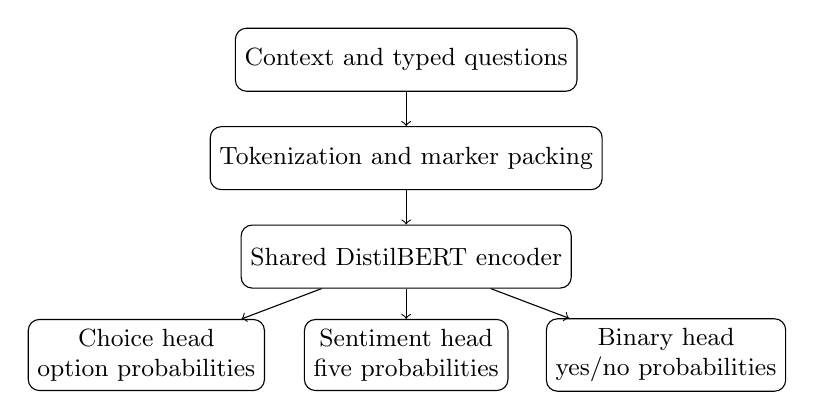
\begin{tikzpicture}[node distance=1.25cm, every node/.style={draw,rounded corners,align=center,font=\small,minimum height=0.8cm}]
\node (input) {Context and typed questions};
\node (tokens) [below of=input] {Tokenization and marker packing};
\node (encoder) [below of=tokens] {Shared DistilBERT encoder};
\node (choice) [below of=encoder,xshift=-3.3cm] {Choice head\\option probabilities};
\node (score) [below of=encoder] {Sentiment head\\five probabilities};
\node (binary) [below of=encoder,xshift=3.3cm] {Binary head\\yes/no probabilities};
\draw[->] (input)--(tokens); \draw[->] (tokens)--(encoder);
\draw[->] (encoder)--(choice); \draw[->] (encoder)--(score); \draw[->] (encoder)--(binary);
\end{tikzpicture}
\caption{Jevlet's system architecture. Marker representations feed typed heads after one packed encoder pass.}
\label{fig:architecture}
\end{figure*}

\subsection{Choice and Binary Heads}
The choice scorer maps every option representation to a scalar,
\begin{equation}
z_{ij}=w_c^\top h_{o_{ij}}+b_c,\qquad
p_{ij}=\frac{\exp(z_{ij}/T_c)}{\sum_{k\in O_i}\exp(z_{ik}/T_c)}.
\end{equation}
Only supplied options participate in the softmax. Unused option slots are masked, and the maximum-probability option is returned as the typed answer. Its probability is relative to the current shortlist.

The binary head reads a question marker and produces
\begin{equation}
p_i(\mathrm{yes})=\sigma((w_b^\top h_{q_i}+b_b)/T_b).
\end{equation}
The no probability is its complement. The predicted answer is a boolean, and confidence is the probability of that predicted answer. Training predicates refer to known banking intents; the interface alone does not establish understanding of arbitrary predicates.

\subsection{Five-Level Sentiment Head}
The categorical head maps the sentiment question marker to five logits:
\begin{equation}
\boldsymbol{p}_i=\operatorname{softmax}((W_s h_{q_i}+b_s)/T_s).
\end{equation}
The levels correspond to very negative, negative, neutral, positive, and very positive review sentiment. The discrete answer is $1+\arg\max_j p_{ij}$, and the expected score is $\sum_{j=1}^{5}j p_{ij}$. The latter retains uncertainty that a single discrete level hides.

The original head instead learns a scalar $s$ and four ordered thresholds $\beta_1<\cdots<\beta_4$, using softplus increments to preserve order. With $u_k=\sigma((s-\beta_k)/T_s)$, the probabilities are $(1-u_1,u_1-u_2,u_2-u_3,u_3-u_4,u_4)$. Narrow threshold spacing can leave intermediate levels weakly represented under argmax. The categorical revision changes both the parameterization and the supervised sentiment loss, so their effects cannot be separated by this ablation alone.

\section{Learning and Expanded Validation}
\subsection{Dataset Description and Supervision}
BANKING77 supplies 77 banking intent labels~\cite{banking}. SST-5 supplies English review sentiment labels~\cite{sst}. Contexts are partitioned before questions are derived. Case-folded, whitespace-normalized duplicate contexts are removed with test taking precedence; the manifest records 15 within-split and 11 cross-split removals. Retained counts appear in Table~\ref{tab:data}.

\begin{table}[t]
\caption{Unique source texts; unchanged across the Jevlet experiments}
\label{tab:data}\centering
\begin{tabular}{lrrr}\toprule
Partition & Banking & Reviews & Total\\\midrule
Training & 7,993 & 8,531 & 16,524\\
Validation & 999 & 550 & 1,549\\
Calibration & 1,000 & 550 & 1,550\\
Test & 3,079 & 2,210 & 5,289\\\bottomrule
\end{tabular}\end{table}

Banking choice questions include the true intent and one to nine sampled alternatives. Yes/no labels are sampled positive with probability 0.5. In packed requests, queried labels occur among the supplied options, removing a simple option-presence shortcut. Training samples choice-only, binary-only, paired, and three-question recipes, with deterministic epoch-wise variation in candidates and question order. The fixed canonical evaluation request has one choice and two binary questions per banking text, or one sentiment question per review.

The choice task evaluates a shortlist containing the correct label, not retrieval over all 77 labels. Binary prevalence is approximately balanced by construction. Banking texts do not supply sentiment labels, and review texts do not supply banking intent labels.

\subsection{Mathematical Objectives and Initial Training}
Choice and categorical sentiment use cross-entropy; binary prediction uses binary cross-entropy. The ordinal sentiment variant uses binary cross-entropy over four cumulative targets. Every question also contributes a Brier penalty $0.5\sum_j(p_j-y_j)^2$. Losses are averaged within each represented head, then across those heads. All heads update the same encoder, so sentiment changes can affect banking performance.

The initial runs use seed 42, AdamW, learning rate $3\times10^{-5}$, weight decay 0.01, 10\% warm-up, gradient clipping at one, batch size eight, and two-step accumulation. They train for at most six epochs, with patience two on validation loss. The categorical variant is chosen using uncalibrated validation sentiment accuracy. Both variants begin from the same pinned pretrained encoder revision.

\subsection{Model Tuning Optimization and Regularization}
The original validation partition was already a collection of 1,549 texts, not a single example. Its review question used one canonical template. We expand its question coverage to five fixed views per source text. Banking views vary question phrasing, candidate sets, and queried predicates; review views use five phrasings of the same sentiment task. This yields 4,995 banking requests and 2,750 review requests: 7,745 requests and 17,735 decisions overall.

Views share their source text and target labels. They are correlated measurements and are not counted as new independent contexts. This protocol is neither five-fold cross-validation nor a larger source dataset. Its purpose is to reduce dependence on one prompt template and one banking shortlist sample.

Further training starts from the earlier five-class checkpoint and samples the same five question templates during training. Three predefined seed/learning-rate settings are tried: $(42,5\times10^{-6})$, $(43,10^{-5})$, and $(44,2\times10^{-5})$. Each has a three-epoch maximum, patience two, and otherwise retains the initial optimizer settings. Within a candidate, the checkpoint maximizes expanded-validation sentiment accuracy. Across candidates, selection uses that accuracy subject to choice and binary accuracy each remaining within one percentage point of the initial checkpoint on expanded validation. The initial checkpoint remains eligible as a fallback.

These are three refinement settings sharing an initialization, not three independent from-scratch estimates of model quality. Fixed validation and canonical test sampling use request seed 42. Test scores are not used to rank the refinement candidates. The selected checkpoint is evaluated after validation selection.


\subsection{Making Predictions}
At inference time, the tokenizer records question and option marker positions, the encoder contextualizes the packed sequence, and the heads produce logits. Calibrated probabilities determine the typed answer. The response returns the question identifier, answer, probability vector, winning confidence, and context truncation count. Sentiment also returns its expected score. These fields allow an application to inspect uncertainty or defer low-confidence decisions; a confidence threshold is not validated as a production safety rule in this study.

\subsection{Calibration, Metrics, and Execution}
One positive temperature per head minimizes negative log-likelihood (NLL) on the separate calibration partition. Fitting uses L-BFGS with a bounded log-temperature for numerical stability. Positive temperature scaling preserves categorical and binary argmax predictions, while the ordinal decoder can change its winning class.

We report accuracy for all heads, intent macro-F1, sentiment macro-F1 and mean absolute error (MAE), and binary AUROC. Probability quality uses 15-bin top-label expected calibration error (ECE), NLL, and summed multiclass Brier error. A model's winning probability is its confidence; it is not a correctness guarantee.

Learned-model training, validation/test forward passes, and temperature optimization use CUDA. CPU routines handle tokenization, summaries, and serialization. The device is an NVIDIA GeForce RTX 4060 Laptop GPU with 8~GiB VRAM. Device memory, utilization, temperature, and power are sampled every ten seconds. GPU form factor affects throughput, power, and memory constraints; it does not intrinsically change the learning objective or guarantee a different accuracy.

\section{Results and Discussion}
\subsection{Jevlet Quality and Validation Selection}
The original ordinal Jevlet attains 35.20\% calibrated sentiment accuracy, while the earlier five-class Jevlet reaches 52.22\%. Its sentiment macro-F1 also rises from 0.2770 to 0.5141. This revision improves intermediate-level coverage, but banking shortlist accuracy changes from 97.04\% to 95.45\%, and binary accuracy changes from 97.99\% to 96.83\%. Shared learning therefore makes the head revision a task-specific tradeoff rather than a universal improvement.

Table~\ref{tab:validation} reports the expanded-validation measurements. The selected checkpoint is seed42\_lr5e-06. Binary accuracy across the five validation views changes from 79.50\% to 96.40\%. This exposes sensitivity to question wording that a canonical-template evaluation can hide. Because the same five forms are sampled in refinement training, the result shows adaptation to known forms rather than unrestricted paraphrase generalization. The selected checkpoint changes canonical test sentiment accuracy from 52.22\% to 51.72\%, a difference of -0.50 percentage points. Its calibrated canonical test results are 95.97\% shortlist accuracy, 51.72\% sentiment accuracy, sentiment macro-F1 0.4929, sentiment MAE 0.5674, and 97.08\% binary accuracy. The test comprises 3,079 choice, 2,210 sentiment, and 6,158 binary decisions.

\begin{table}[t]
\caption{Expanded-validation accuracy (\%); five correlated views per text. Seed and learning rate identify refinement settings.}
\label{tab:validation}\centering\footnotesize\setlength{\tabcolsep}{3pt}
\begin{tabular}{lrrr}\toprule
Checkpoint & Choice & Sentiment & Binary\\\midrule
Initial five-class & 93.45 & 49.13 & 79.50 \\
seed42\_lr5e-06 & 94.95 & 50.25 & 96.40 \\
seed43\_lr1e-05 & 96.08 & 49.53 & 96.94 \\
seed44\_lr2e-05 & 95.78 & 49.20 & 97.12 \\
\bottomrule\end{tabular}\end{table}

\subsection{External Comparisons}
To place Jevlet's measured quality in context, Table~\ref{tab:comparison} includes GPU-trained TF-IDF logistic and squared-hinge linear classifiers~\cite{svm}, as well as conventional DistilBERT, BERT, and RoBERTa classifiers~\cite{roberta}. They use the same source partitions and canonical test requests. Context classifiers read text alone and produce 77 intent logits, five sentiment logits, and 77 binary predicate logits. Supplied label IDs select shortlist and binary outputs; they do not interpret arbitrary question text.

TF-IDF uses training-fitted unigrams/bigrams, sublinear term frequency, and at most 20,000 features. Its linear classifiers are optimized with CUDA PyTorch operations, not a dedicated library SVM solver. The logistic objective includes the same Brier penalty; the SVM uses squared one-vs-rest hinge loss without that term. Linear models have a 40-epoch maximum, batch size 256, learning rate 0.01, and patience five. Transformer classifiers have the initial six-epoch budget. Checkpoints use validation loss, and temperatures use separate calibration data.

\begin{table*}[t]
\caption{Calibrated canonical test results. Accuracies are percentages. Jevlet refinement has additional tuning exposure; the table is not an equal-compute comparison.}
\label{tab:comparison}\centering\footnotesize\setlength{\tabcolsep}{3pt}
\begin{tabular}{lrrrrr}\toprule
Model & Choice \% & Sent. \% & Sent. F1 & MAE & Binary \%\\\midrule
Jevlet (ordinal) & 97.04 & 35.20 & 0.2770 & 0.8584 & 97.99 \\
Jevlet (five-class) & 95.45 & 52.22 & 0.5141 & 0.5724 & 96.83 \\
TF-IDF + logistic & 97.86 & 39.86 & 0.3754 & 0.8394 & 95.96 \\
TF-IDF + linear SVM & 97.76 & 39.77 & 0.3736 & 0.8516 & 95.73 \\
DistilBERT classifier & 97.21 & 49.23 & 0.4324 & 0.5837 & 89.48 \\
BERT-base classifier & 97.08 & 53.12 & 0.4875 & 0.5443 & 90.40 \\
RoBERTa-base classifier & 97.73 & 54.12 & 0.4782 & 0.5059 & 93.28 \\
Jevlet (refined, selected) & 95.97 & 51.72 & 0.4929 & 0.5674 & 97.08 \\
\bottomrule\end{tabular}\end{table*}

The selected Jevlet has the highest sentiment macro-F1 among the evaluated external configurations. Its typed interface combines these decisions in one checkpoint and supports packed questions. The highest external sentiment accuracy is 54.12\%, obtained by RoBERTa-base classifier. A larger exact-level accuracy and a larger macro-F1 can favor different models because class coverage matters. The table therefore supports specific strengths rather than a claim that Jevlet wins every task.

Source contexts and label decisions are matched, but inputs and optimization differ. Jevlet shares 256 tokens between questions and context, whereas the context classifiers allocate that budget to text alone and use fixed label identities. Tokenization, truncation, task objectives, and tuning budgets differ. Jevlet's additional refinement cannot be treated as a controlled encoder-only ablation. The original comparator runs use one seed; their scores do not establish optimally tuned baselines.

\begin{figure}[t]
\centering
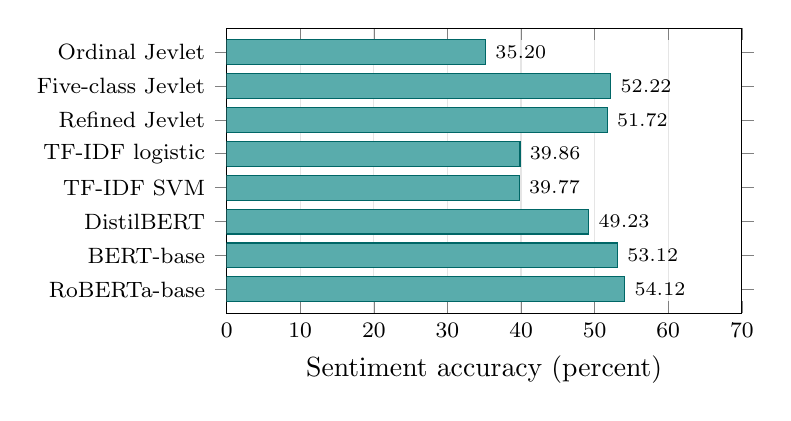
\begin{tikzpicture}
\begin{axis}[xbar,width=0.67\columnwidth,height=5.2cm,xmin=0,xmax=70,
ytick={0,1,2,3,4,5,6,7},yticklabels={Ordinal Jevlet,Five-class Jevlet,Refined Jevlet,TF-IDF logistic,TF-IDF SVM,DistilBERT,BERT-base,RoBERTa-base},
y dir=reverse,xlabel={Sentiment accuracy (percent)},bar width=9pt,enlarge y limits=0.1,
nodes near coords,nodes near coords align={horizontal},
every node near coord/.append style={font=\scriptsize,/pgf/number format/fixed,
/pgf/number format/precision=2,/pgf/number format/fixed zerofill},tick label style={font=\footnotesize},
xmajorgrids=true,grid style={gray!20}]
\addplot[fill=teal!65,draw=teal!80!black] coordinates {(35.2036,0) (52.2172,1) (51.7195,2) (39.8643,3) (39.7738,4) (49.2308,5) (53.1222,6) (54.1176,7)};
\end{axis}\end{tikzpicture}
\caption{Sentiment accuracy (percent) on the shared canonical test set. Additional refinement tuning and differing model inputs prevent an equal-compute architectural claim.}
\end{figure}
\begin{figure}[t]
\centering
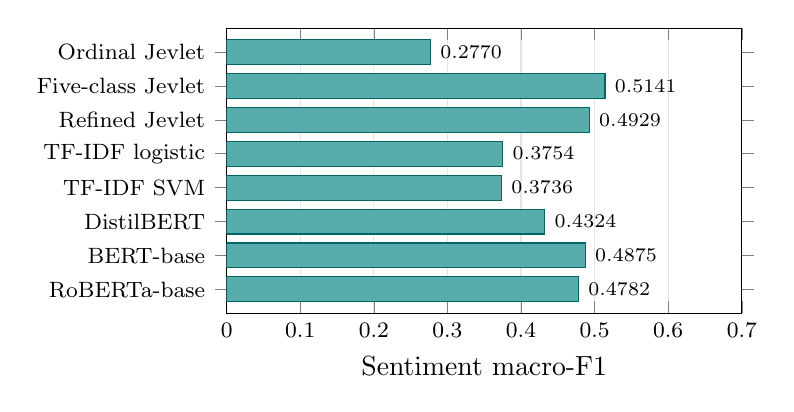
\begin{tikzpicture}
\begin{axis}[xbar,width=0.67\columnwidth,height=5.2cm,xmin=0,xmax=0.7,
ytick={0,1,2,3,4,5,6,7},yticklabels={Ordinal Jevlet,Five-class Jevlet,Refined Jevlet,TF-IDF logistic,TF-IDF SVM,DistilBERT,BERT-base,RoBERTa-base},
y dir=reverse,xlabel={Sentiment macro-F1},bar width=9pt,enlarge y limits=0.1,
nodes near coords,nodes near coords align={horizontal},
every node near coord/.append style={font=\scriptsize,/pgf/number format/fixed,
/pgf/number format/precision=4,/pgf/number format/fixed zerofill},tick label style={font=\footnotesize},
xmajorgrids=true,grid style={gray!20}]
\addplot[fill=teal!65,draw=teal!80!black] coordinates {(0.2770,0) (0.5141,1) (0.4929,2) (0.3754,3) (0.3736,4) (0.4324,5) (0.4875,6) (0.4782,7)};
\end{axis}\end{tikzpicture}
\caption{Sentiment macro-F1 on the shared canonical test set. Additional refinement tuning and differing model inputs prevent an equal-compute architectural claim.}
\end{figure}
\subsection{Calibration and Confidence}
Table~\ref{tab:calibration} reports the selected Jevlet before and after temperature fitting. Discrete categorical predictions remain unchanged by temperature scaling, so any categorical accuracy change is attributable to the trained checkpoint rather than to this post-processing step. ECE, NLL, and Brier error measure different aspects of confidence, and a temperature fitted to calibration-set NLL need not minimize every test metric.

\begin{table*}[t]
\caption{Selected Jevlet probability quality before (B) and after (A) calibration; lower values are better.}
\label{tab:calibration}\centering\small
\begin{tabular}{lrrrrrr}\toprule
Head & ECE B & ECE A & NLL B & NLL A & Brier B & Brier A\\\midrule
Choice & 0.0158 & 0.0073 & 0.1304 & 0.1198 & 0.0629 & 0.0614 \\
Sentiment & 0.2150 & 0.0344 & 1.3051 & 1.1039 & 0.6699 & 0.5997 \\
Binary & 0.0142 & 0.0063 & 0.0979 & 0.0924 & 0.0484 & 0.0473 \\
\bottomrule\end{tabular}\end{table*}

\subsection{Packed Prediction Cost}
Table~\ref{tab:timing} measures the selected checkpoint on fixed three-question banking requests. Packed mode uses one sequence per context. Sequential mode uses three passes; batched-question mode sends separate question sequences together. All three modes retain the same context tokens. Timing includes probability construction, five warm-up iterations, twenty measured repetitions, and CUDA synchronization. Batch-32 times are amortized milliseconds per request, not individual response latency.

\begin{table}[t]
\caption{Selected Jevlet CUDA float32 median inference time (ms/request). Complete time includes packing and transfer.}
\label{tab:timing}\centering\footnotesize
\begin{tabular}{lrrr}\toprule
Mode & Batch & Forward & Complete\\\midrule
Packed & 1 & 2.75 & 3.35 \\
Packed & 32 & 1.82 & 2.20 \\
Sequential & 1 & 8.88 & 10.18 \\
Sequential & 32 & 2.82 & 3.78 \\
Batched questions & 1 & 3.52 & 4.26 \\
Batched questions & 32 & 4.73 & 5.47 \\
\bottomrule\end{tabular}\end{table}

For batch one, packed forward time is 2.75~ms and sequential forward time is 8.88~ms. This matched workload demonstrates the effect of avoiding repeated encoding within Jevlet. It does not isolate encoder arithmetic from probability selection, establish service throughput under concurrency, or prove a speedup over every context-only classifier. Preprocessing, sequence length, padding, and thermal conditions influence application-level time.

\section{Limitations and Future Work}
Expanded validation increases coverage of known question templates and banking candidates, not the number of independent contexts. Five paraphrases of one label task do not establish broad prompt understanding. The refinement settings share the same earlier checkpoint, and their seed/learning-rate pairs vary together, so they cannot separate either factor or quantify independent training-seed uncertainty.

Earlier test results were inspected during sentiment diagnosis. Although the refinement search ranks candidates only on validation data, the study remains exploratory. Fresh held-out data, repeated from-scratch runs, and a separately tuned comparator protocol are needed for stronger conclusions. No accuracy gain is guaranteed by simply adding validation requests.

Banking choices contain the true label, and binary queries are approximately balanced. Production shortlists may omit the intent or have a different query prevalence. Sentiment supervision comes only from English reviews; bank-domain sentiment, unseen labels, other languages, and out-of-domain confidence are not established. Multiple questions and repeated validation views share contexts and are correlated. Future work should test these shifts, quantify class-specific errors, and examine task balancing that improves sentiment without sacrificing banking quality.

\section{Conclusion}
Jevlet provides typed choice, sentiment, and binary predictions through one shared encoder and explicit probability outputs. Marker-based packing lets several questions reuse the same text representation. The five-class head addresses a practical weakness of the earlier ordinal sentiment decoder, and expanded validation checks several question forms without confusing repeated views with new labeled examples. The selected checkpoint reaches 51.72\% sentiment accuracy and macro-F1 0.4929 alongside 95.97\% banking shortlist and 97.08\% binary accuracy. The selected Jevlet has the highest sentiment macro-F1 among the evaluated external configurations. Its value is supported by those measured task strengths and a unified interface; universal superiority is not established. Fresh-data evaluation and stronger task balancing remain necessary to assess how well these benefits generalize.

\begin{thebibliography}{10}
\bibitem{distilbert}V. Sanh, L. Debut, J. Chaumond, and T. Wolf, ``DistilBERT, a distilled version of BERT: Smaller, faster, cheaper and lighter,'' \emph{arXiv preprint arXiv:1910.01108}, 2019. [Online]. Available: \url{https://arxiv.org/abs/1910.01108}
\bibitem{bert}J. Devlin, M.-W. Chang, K. Lee, and K. Toutanova, ``BERT: Pre-training of deep bidirectional transformers for language understanding,'' in \emph{Proc. NAACL-HLT}, 2019, pp. 4171--4186, doi: 10.18653/v1/N19-1423.
\bibitem{laya}N. Mukkunnoth and Convai Innovations, ``Laya: Non-autoregressive System 1 decision engine,'' GitHub repository. Accessed: Oct. 11, 2026. [Online]. Available: \url{https://github.com/NandhaKishorM/laya}
\bibitem{coral}W. Cao, V. Mirjalili, and S. Raschka, ``Rank consistent ordinal regression for neural networks with application to age estimation,'' \emph{Pattern Recognition Letters}, vol. 140, pp. 325--331, 2020. [Online]. Available: \url{https://arxiv.org/abs/1901.07884}
\bibitem{guo}C. Guo, G. Pleiss, Y. Sun, and K. Q. Weinberger, ``On calibration of modern neural networks,'' in \emph{Proc. 34th Int. Conf. Machine Learning}, vol. 70, 2017, pp. 1321--1330. [Online]. Available: \url{https://proceedings.mlr.press/v70/guo17a.html}
\bibitem{brier}G. W. Brier, ``Verification of forecasts expressed in terms of probability,'' \emph{Monthly Weather Review}, vol. 78, no. 1, pp. 1--3, 1950.
\bibitem{banking}I. Casanueva, T. Temcinas, D. Gerz, M. Henderson, and I. Vuli\'{c}, ``Efficient intent detection with dual sentence encoders,'' in \emph{Proc. 2nd Workshop on Natural Language Processing for Conversational AI}, 2020, pp. 38--45, doi: 10.18653/v1/2020.nlp4convai-1.5.
\bibitem{sst}R. Socher, A. Perelygin, J. Wu, J. Chuang, C. D. Manning, A. Ng, and C. Potts, ``Recursive deep models for semantic compositionality over a sentiment treebank,'' in \emph{Proc. EMNLP}, 2013, pp. 1631--1642. [Online]. Available: \url{https://aclanthology.org/D13-1170/}
\bibitem{svm}C. Cortes and V. Vapnik, ``Support-vector networks,'' \emph{Machine Learning}, vol. 20, pp. 273--297, 1995, doi: 10.1007/BF00994018.
\bibitem{roberta}Y. Liu et al., ``RoBERTa: A robustly optimized BERT pretraining approach,'' \emph{arXiv preprint arXiv:1907.11692}, 2019. [Online]. Available: \url{https://arxiv.org/abs/1907.11692}
\end{thebibliography}
\end{document}
